\documentclass{beamer}

\usepackage{graphicx}

\setbeamertemplate{navigation symbols}{}

\begin{document}
\begin{frame}[fragile]
\verb|[H]c1c(c(c2=NON=c2c1[H])C3(C(=C(N(C(=C3[|
\verb|H])[H])[H])[H])[H])[H])[H]|

\begin{figure}
    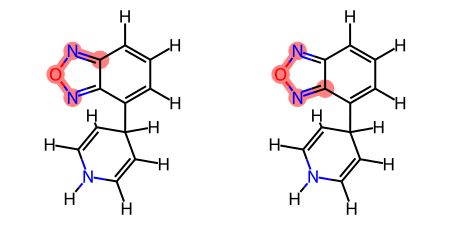
\includegraphics[width=0.7\textwidth,height=0.7\textheight,keepaspectratio]{mol00.png}
\end{figure}
\end{frame}
\begin{frame}[fragile]
\verb|[H]c1c(c(c2=NON=c2c1[H])C3(C(=C(N(C(=C3[|
\verb|H])[H])[H])[H])[H])[H])[H]|

\begin{figure}
    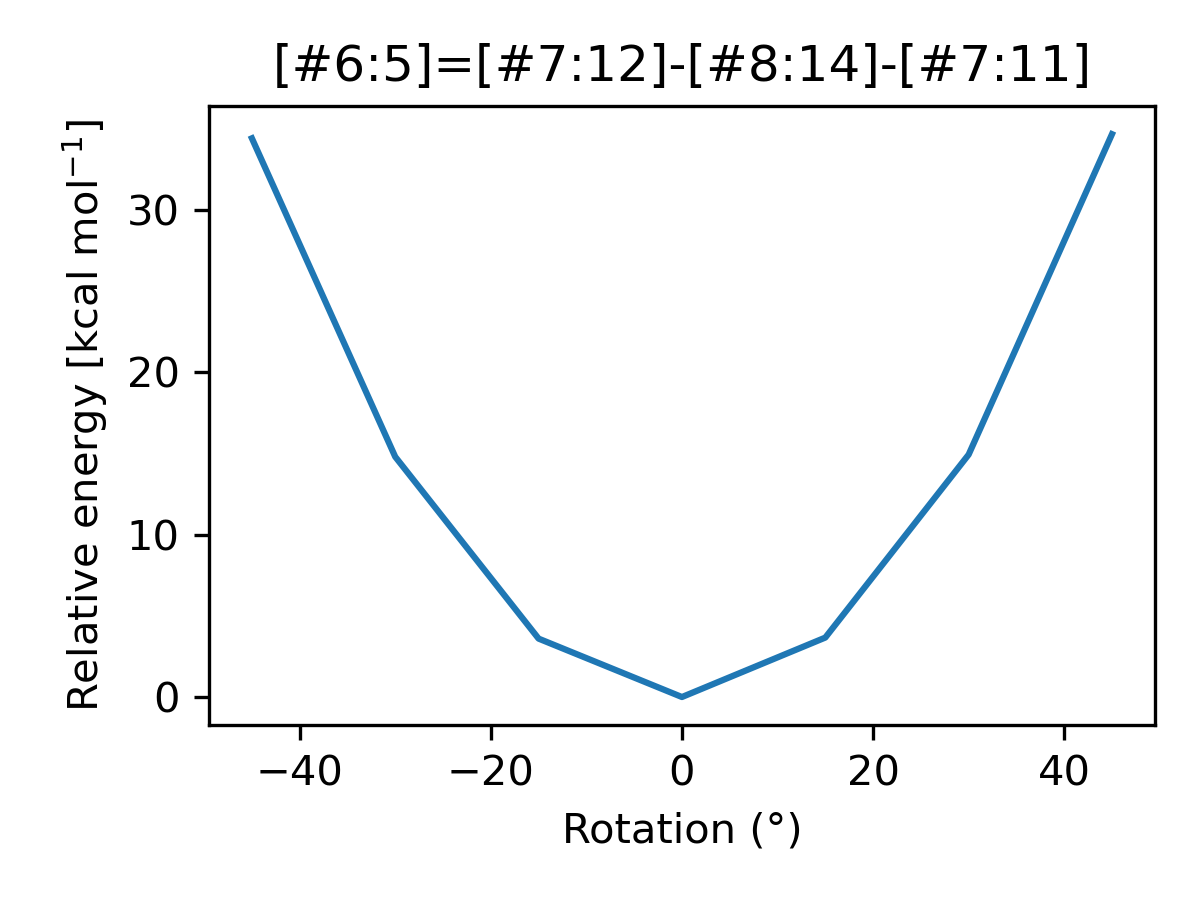
\includegraphics[width=0.7\textwidth,height=0.7\textheight,keepaspectratio]{plot00.png}
\end{figure}
\end{frame}
\begin{frame}[fragile]
\verb|[H]c1c(c(c(c(c1/N=N/C2=C(ON=C2C([H])([H]|
\verb|)[H])C([H])([H])[H])[H])[H])OC([H])([H])|
\verb|[H])[H]|

\begin{figure}
    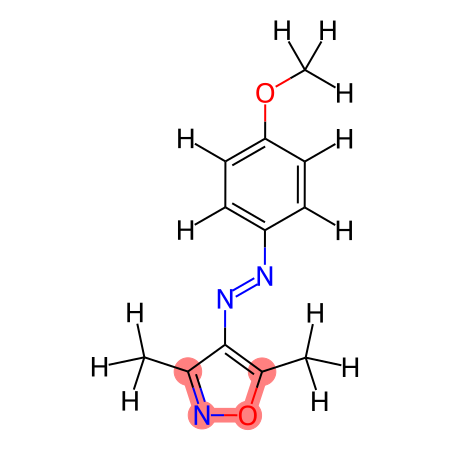
\includegraphics[width=0.7\textwidth,height=0.7\textheight,keepaspectratio]{mol06.png}
\end{figure}
\end{frame}
\begin{frame}[fragile]
\verb|[H]c1c(c(c(c(c1/N=N/C2=C(ON=C2C([H])([H]|
\verb|)[H])C([H])([H])[H])[H])[H])OC([H])([H])|
\verb|[H])[H]|

\begin{figure}
    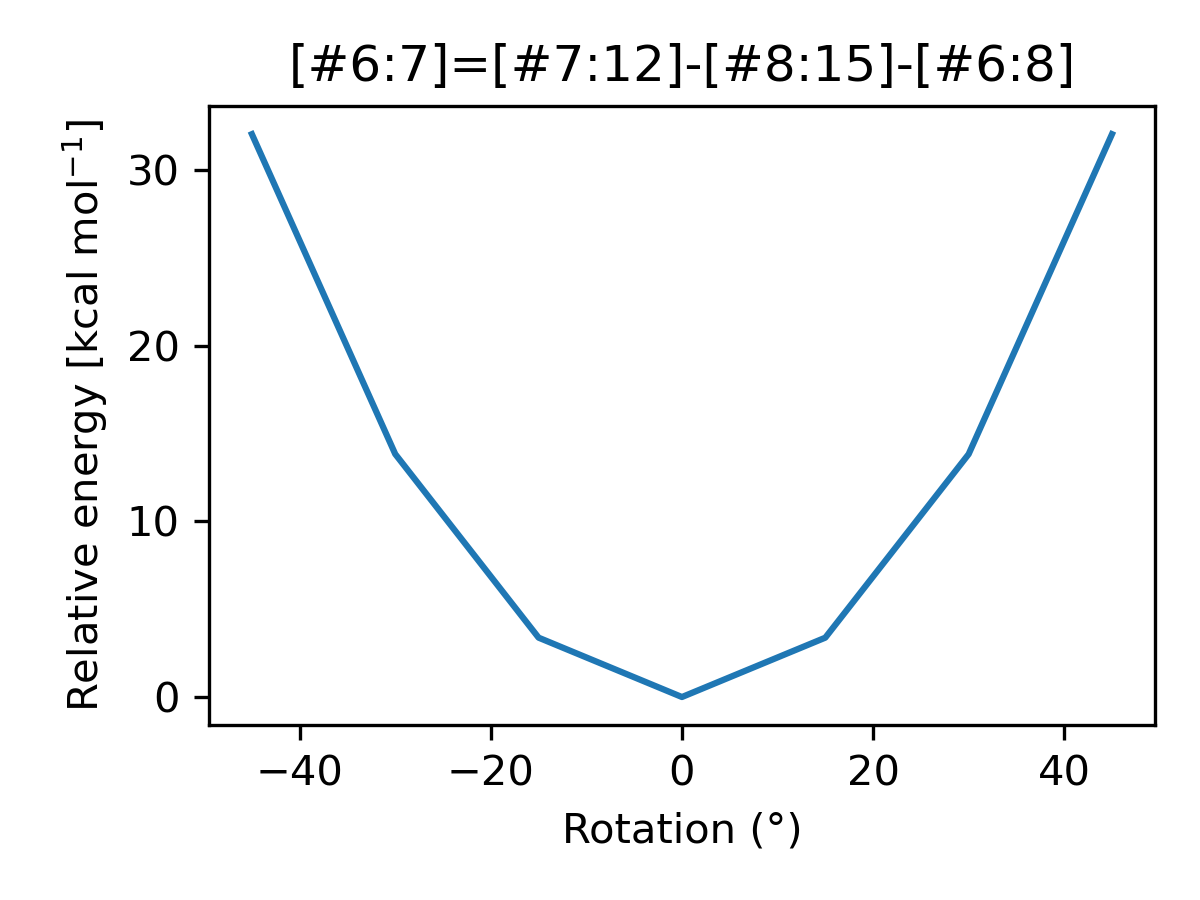
\includegraphics[width=0.7\textwidth,height=0.7\textheight,keepaspectratio]{plot06.png}
\end{figure}
\end{frame}
\begin{frame}[fragile]
\verb|[H]C1=C(SC(=C1[H])C2=C(C(=NO2)C([H])([H]|
\verb|)[H])C([H])([H])C(=O)O[H])[H]|

\begin{figure}
    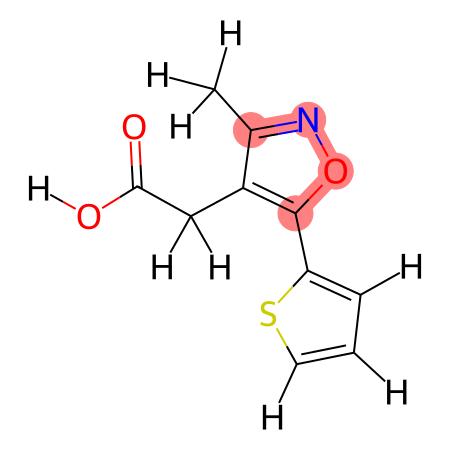
\includegraphics[width=0.7\textwidth,height=0.7\textheight,keepaspectratio]{mol07.png}
\end{figure}
\end{frame}
\begin{frame}[fragile]
\verb|[H]C1=C(SC(=C1[H])C2=C(C(=NO2)C([H])([H]|
\verb|)[H])C([H])([H])C(=O)O[H])[H]|

\begin{figure}
    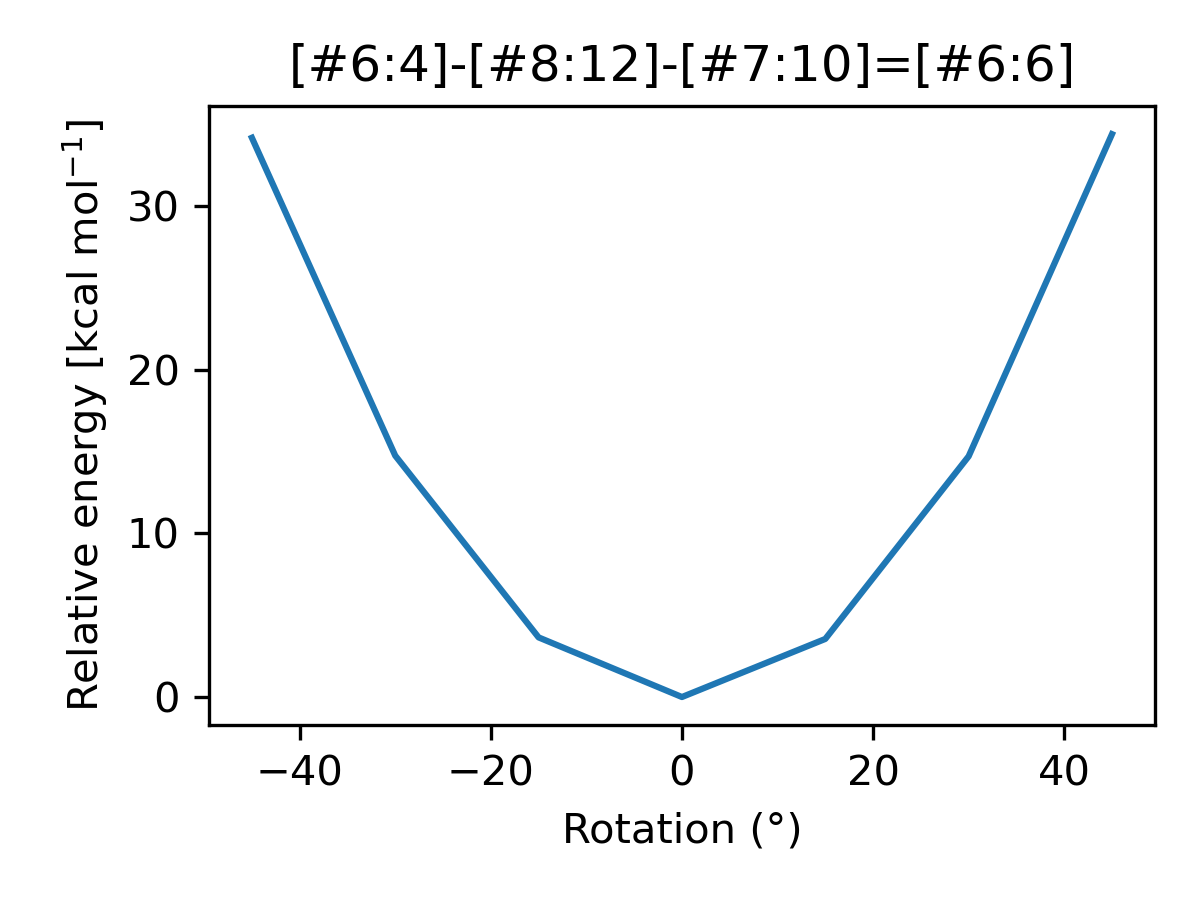
\includegraphics[width=0.7\textwidth,height=0.7\textheight,keepaspectratio]{plot07.png}
\end{figure}
\end{frame}
\begin{frame}[fragile]
\verb|[H]c1c(c(c(c(c1[H])[H])C2=NOC3(C2=O)C(C(|
\verb|C(C(C3([H])[H])([H])[H])([H])[H])([H])[H|
\verb|])([H])[H])[H])[H]|

\begin{figure}
    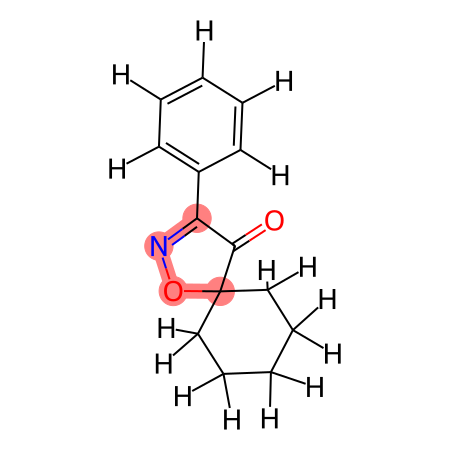
\includegraphics[width=0.7\textwidth,height=0.7\textheight,keepaspectratio]{mol08.png}
\end{figure}
\end{frame}
\begin{frame}[fragile]
\verb|[H]c1c(c(c(c(c1[H])[H])C2=NOC3(C2=O)C(C(|
\verb|C(C(C3([H])[H])([H])[H])([H])[H])([H])[H|
\verb|])([H])[H])[H])[H]|

\begin{figure}
    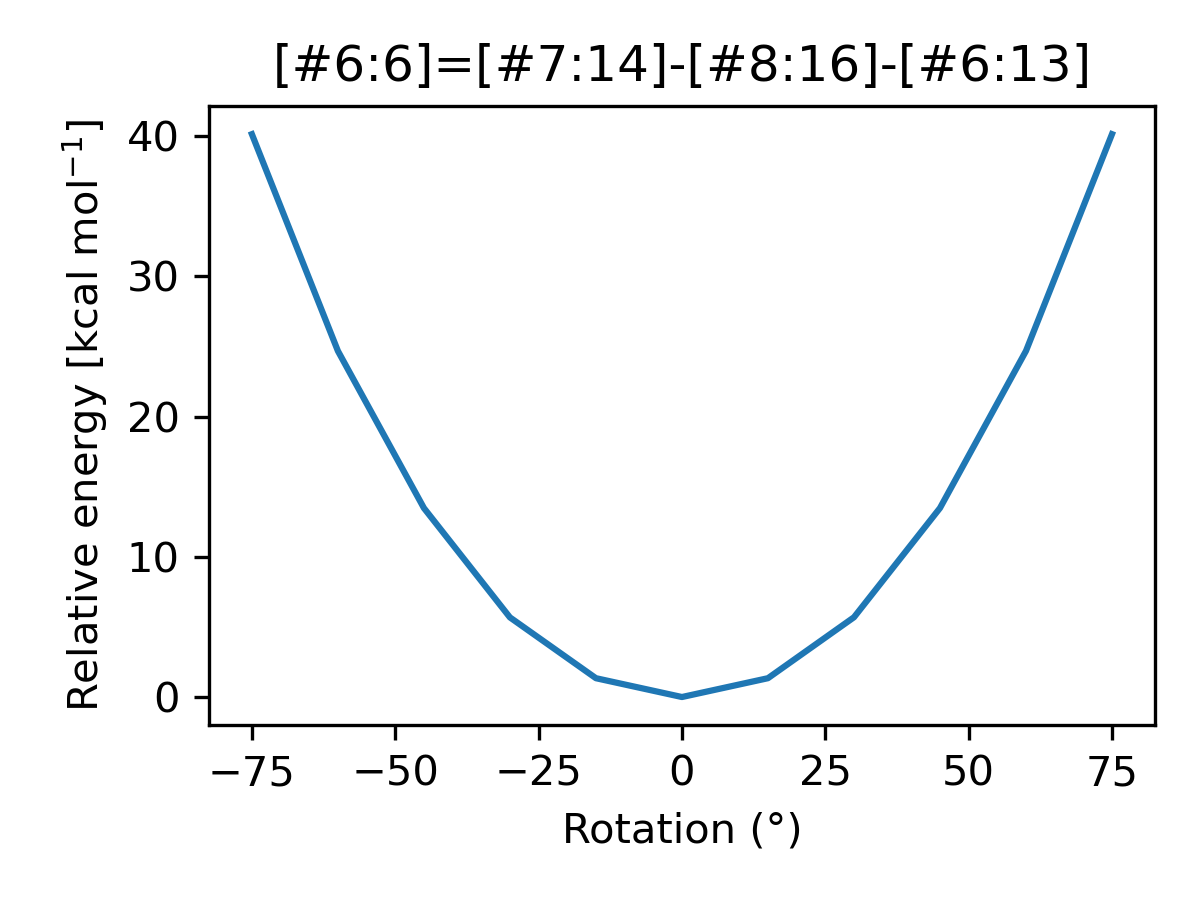
\includegraphics[width=0.7\textwidth,height=0.7\textheight,keepaspectratio]{plot08.png}
\end{figure}
\end{frame}
\begin{frame}[fragile]
\verb|[H]c1c(c(c(c2c1N3C(=NC(=C3C(N(C2=O)C([H]|
\verb|)([H])[H])([H])[H])C4=NC(=NO4)C([H])([H]|
\verb|)C([H])([H])[H])[H])[H])Cl)[H]|

\begin{figure}
    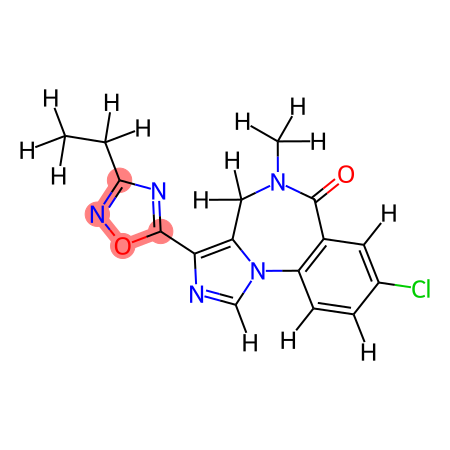
\includegraphics[width=0.7\textwidth,height=0.7\textheight,keepaspectratio]{mol10.png}
\end{figure}
\end{frame}
\begin{frame}[fragile]
\verb|[H]c1c(c(c(c2c1N3C(=NC(=C3C(N(C2=O)C([H]|
\verb|)([H])[H])([H])[H])C4=NC(=NO4)C([H])([H]|
\verb|)C([H])([H])[H])[H])[H])Cl)[H]|

\begin{figure}
    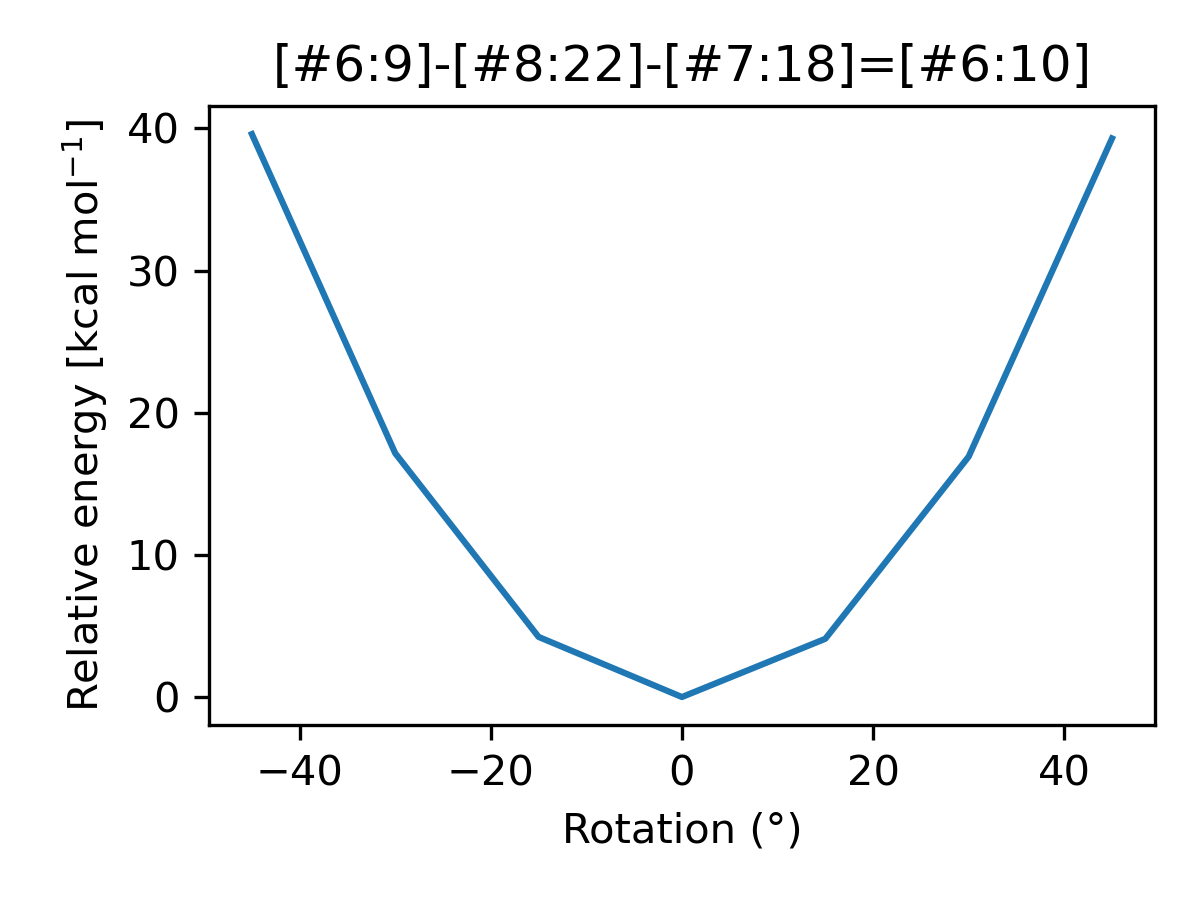
\includegraphics[width=0.7\textwidth,height=0.7\textheight,keepaspectratio]{plot10.png}
\end{figure}
\end{frame}
\end{document}